\documentclass[10pt]{article}

\usepackage{amsmath}
\usepackage{amssymb}
\usepackage{array}
\usepackage{tabu}
\usepackage{lmodern}
\usepackage{graphicx}
\usepackage[space]{grffile}
\usepackage{subfigure}
\usepackage{longtable}
\usepackage{multirow}
\usepackage[margin=1.0in]{geometry}
\renewcommand{\baselinestretch}{2.0}

%\usepackage[font=small,labelfont=bf,labelsep=period]{caption}
\usepackage[style=authoryear,sorting=nyt,url=false,isbn=false,doi=false,firstinits=true,backend=biber]{biblatex}

\renewcommand{\baselinestretch}{2.0}
\renewcommand*\contentsname{Table of Contents}
%\captionsetup{font={stretch=2.0}}

\DeclareNameAlias{default}{last-first}

\DefineBibliographyStrings{english}{%
	andothers = {\addcomma\addspace\textsc{et\addabbrvspace al}\adddot},
	and = {\textsc{and}}
}
\renewcommand*{\labelnamepunct}{\space\space}

\renewbibmacro{in:}
{%
	\ifentrytype{article}{%
	}{%
		\printtext{\bibstring{in}\intitlepunct}%
	}%
}
\renewbibmacro*{volume+number}{%
	\printfield{volume}%
	\setunit*{\addcomma\space}%
	\printfield{number}%
	\setunit{\addcomma\space}}

\DeclareFieldFormat{pages}{#1}

\renewbibmacro*{publisher+location+date}{%
	\printlist{publisher}%
	\setunit*{\addcomma\space}%
	\printlist{location}%
	\setunit*{\addcomma\space}%
	\usebibmacro{date}%
	\newunit}

\renewcommand{\newunitpunct}{\addcomma\space}
\DeclareFieldFormat[article,inbook,incollection,inproceedings,patent,thesis,unpublished]{title}{#1} 
\DeclareFieldFormat{year}{#1} 

\addbibresource{refs/ident_refs.bib}

\begin{document}
\paragraph{Outline:}
\begin{itemize}
	\item Importance of parameter values for estimating in vivo response using kinetic models of metabolism and consequently for metabolic network design using kinetic models of metabolism
	\item The need for parameter identifiability to determine unique and true parameter values from observed data
	\item Types and purpose of identifiability for parameters
	\item Methods for structural identifiability and existing methods for practical identifiability
	\item Lack of methods for practical identifiability and consequently experimental design (not covered?)
	\item work done in this paper for practical identifiability			
	\item scalability of computer algebra-based methods for structural identifiability (using CRNT to reduce networks to make structural identifiability scalable) (move to discussion - may be in discussion)
\end{itemize}
\section{Introduction:}
Kinetic models of metabolism can be used to study the dynamic characteristics of metabolic networks. In these models, ordinary differential equations (ode) are used to express the rate of change of metabolite concentrations ($x$) as a function of the reaction fluxes ($v$) in the metabolic network (Equation \ref{eq:kinstoich}). The matrix $\mathbf{S}$ in Equation (\ref{eq:kinstoich}a) defines the stoichiometric relationship between the fluxes and the concentrations of the metabolic network.
\begin{subequations}\label{eq:kinstoich}
	\begin{align}
	\dot{x} = \mathbf{S}v\\
	v = g(x, \theta, u)
	\end{align}
\end{subequations}
The expression for the nonlinear function ($g$) used to describe each reaction flux $v_i$ in a kinetic model (Equation \ref{eq:kinstoich}b) is dependent on the enzyme kinetic mechanism that is used to model the reaction (older kinetic modeling papers, reviews, Srinivasan et al., 2015). Accordingly, $g$ is a nonlinear function of the metabolite concentrations, enzyme kinetic parameters ($\theta$) and other input concentrations ($u$). 

The ability to predict the steady state and dynamic responses of metabolic networks, under in vivo conditions, to different perturbations is dependent on the numerical values of the enzyme kinetic parameter values ($\theta$) in Equation (\ref{eq:kinstoich}). Analyzing the ability of a metabolic network to exhibit dynamic characteristics like multiple steady states and oscillations, irrespective of the structure of the network, is one example where parameter values might play a crucial role (Srinivasan et al., 2017?). The use of in vitro, or unreliable in vivo parameter estimates, reduces confidence in the model predicted behaviour. Consequently, the reduction in confidence hampers the use of these models to gain insight into the functioning of metabolic networks (ensemble modeling and ORACLE papers). The insights gained from the use of kinetic models are subsequently used to design changes to these metabolic networks to achieve various goals. These goals could either be to increase metabolite production for biosynthesis of different chemicals (kinetic model for BDO in ecoli, k-ecoli457, Srinivasan et al., 2017) or to find therapeutic targets that can cut-off metabolic pathways to kill cancer cells (new paper on using geneMCS for cancer cell lines). Hence, an increase in uncertainty in model predicted responses is also an obstacle for using the predicted responses as a basis for designing the metabolic networks to achieve these goals.  

If all intracellular metabolite concentrations can be measured over a time course, and the corresponding data is available, a nonlinear programming problem can be formulated to estimate the enzyme kinetic parameters ($\theta$) in Equation (\ref{eq:kinstoich}). The minimization of least square error between the measured ($x^*$) and modeled ($x$) concentrations can be used as an objective function (Equation \ref{eq:lsqopt}a) for the optimization problem (Equation \ref{eq:lsqopt}), with fixed upper ($\theta_u$) and lower ($\theta_l$) bounds for the parameter values (Equation \ref{eq:lsqopt}b). The difference between the data and the model estimate for each output and at each time point in the objective function is weighted by the variance in the experimental data $\sigma_{kl}^*$ for that corresponding variable and time point.
\begin{subequations}\label{eq:lsqopt}
	\begin{align}
	\underset{\theta}{\mathrm{min}} &\sum_{k=1}^{m}\sum_{l=1}^{d}\left(\frac{x_{kl}^*-x_{kl}}{\sigma_{kl}^*}\right)^2\\
	&\theta_l \le \theta \le \theta_u
	\end{align}
\end{subequations}

However, not all metabolite concentrations used in the model (Equation \ref{eq:kinstoich}) can be measured. Additionally, measurable fluxes in the metabolic network also need to be included as part of the parameter estimation problem. In such scenarios, the parameter estimation problem is modified to suit a new system of equations shown below (Equation \ref{eq:output}). The new system of equations is obtained by augmenting the original system (Equation \ref{eq:kinstoich}) with Equation (\ref{eq:output}c) that models the relationship between the measurable metabolite concentrations and fluxes, represented by the variable $y$, and the unmeasured concentrations ($x$) that are used in the original model (Equation \ref{eq:kinstoich}) above. Equation (\ref{eq:output}) now has additional parameters $\mu$ that define this relationship and also need to be estimated.
\begin{subequations}\label{eq:output}
	\begin{align}
	\dot{x} = \mathbf{S}v\\
	v = g(x, y, \theta, u)\\
	\dot{y} = h(x, y, \mu, u)
	\end{align}
\end{subequations}
In systems identification, the measured concentrations and fluxes, $y$ in Equation (\ref{eq:output}c), are called output or observed variables, and the unmeasured concentrations, $x$ in Equation (\ref{eq:output}a-b), are called the state variables. 
For estimating both $\theta$ and $\mu$, the metabolite concentrations ($x$) in the optimization problem (Equation \ref{eq:lsqopt}) are substituted with the output variables $y$. 

However, the ability to determine unique solutions to parameters $\theta$ and $\mu$ is governed by the identifiability of these parameters in the model \parencite{McLean2012}. The identifiability of parameters in nonlinear models can be classified into two categories: structural (or a priori) and practical (or posterior) identifiability. 	
Any system (Equation \ref{eq:output}) is said to be structurally identifiable if, for an input-output mapping defined by $\mathbf{y} = \Phi(\mu,u)$ for at least one input function $u$, any two values of parameters $\mathbf{\mu}_1$ and $\mathbf{\mu}_2$ satisfy the relationship in Equation (\ref{eq:stident}) below.
\begin{align}\label{eq:stident}
\Phi(\mathbf{\mu}_1,u) = \Phi(\mathbf{\mu}_2,u) \iff \mathbf{\mu}_1 = \mathbf{\mu}_2
\end{align}
Accordingly, any system that has an infinite number of solutions to the parameter estimation problem for all input functions is said to structurally non-identifiable. Thus, the structural identifiability of parameters in a dynamic model helps establish the presence or absence of a relationship between the unobservable state variables and the observable output variables. Accordingly, the effect of model structure and parameterization on the ability to infer true parameter values from experimental data is determined by the structural identifiability of the parameter. 

Experimental data from many physical systems is usually noisy, and when parameters are estimated on the basis of noisy data, the ability to estimate unique parameter values to satisfy Equation (\ref{eq:stident}) is referred to as practical identifiability. The effect of the available experimental data on the ability to estimate unique parameter values is determined by the practical identifiability of the parameter. Accordingly, practical identifiability of a parameter is contingent upon the nature, quality and quantity of data available to estimate the parameter as opposed to the structure and parameterization of the model. 

Thus, on the one hand, establishing the structural identifiability of parameters enables one to propose models that are not only appropriate representations of physical processes, but also are parameterized in such a way that the value of these parameters can be estimated. On the other hand, establishing practical identifiability of parameters in any model helps design experiments that are minimal, informative and useful for parameter estimation.

Algorithms have been extensively developed for establishing structural identifiability of dynamic models of biological systems (IEEE Trans paper from 2007). Most of these algorithms use methods based on differential algebra (Glad and Ljung, 1994). More recent methods take a profile-likelihood-based approach (2012 Paper) to establish both structural and practical identifiability. However, these methods scale poorly with increase in size of the modeled system. The aforementioned methods are also heavily dependent on the availability of dynamic time course data for all the output variables of the system. 

Computational burden due to poor scalability can be partly addressed with the current increases in computational power, while current improvements in measuring technologies can enable one to obtain high frequency dynamic data, no scalable methodologies exist to utilize the abundantly available steady state data for parameter estimation and identifiability for large metabolic networks. 

In this paper, we propose a methodology to establish practical identifiability for parameters in kinetic models of metabolism. We present a computer algebra-based method that can facilitate practical identifiability as well as experimental design for estimating parameters separately for each individual reaction within a metabolic network based on available steady state experimental data. This enables us to address the twin issues of scalability and data availability. We illustrate the utility of this method by applying it for a small network of gluconeogenesis in \textit{E. coli} and demonstrating our ability to propose experiments that will facilitate parameter estimation for a kinetic model of this network. We also demonstrate the scalability of the proposed methodology to facilitate experimental design by applying it to a relatively larger metabolic network of the human red blood cell hepatocyte. 	

\section{Methods:}	
\subsection{A method for practical identifiability of kinetic models of metabolism:}\label{sec:ident}
In this section, we show how practical identifiability of kinetic parameters in a dynamic model of metabolism can be established using the nonlinear algebraic kinetic rate law formulations that describe the relationship between the concentrations, fluxes and the kinetic parameters of the metabolic network model. A summary of the methodology in the form of a flow diagram is shown in Figure \ref{fig:ident-flowchart}.
In a kinetic model, the value of every flux $v_i$ is expressed using one of the many available enzyme kinetic formulations. Without loss of generality, all of these kinetic formulations can be expressed as nonlinear algebraic equations (Equation \ref{eq:flux_gen}). The fluxes are expressed as a function of the metabolite concentrations $\mathbf{x}$ and the kinetic parameters $\theta$ (Figure \ref{fig:ident-flowchart}a). 
\begin{align}\label{eq:flux_gen}
v_i = f(\mathbf{x},\mathbf{\theta}, u)
\end{align}
Let $\theta \in \mathbb{R}^p$ for each flux $v_i$ in the network. For each experiment $j = {1, 2, ..., n}$, we assume that all metabolite concentrations $\mathbf{x}$ and reaction fluxes $\mathbf{v}$ are measurable. The pertinent information for each experiment is available as a vector of concentrations and fluxes, $\mathbf{x}_j$ and $\mathbf{v}_j$, respectively (Figure \ref{fig:ident-flowchart}b). 

In order to establish the identifiability of kinetic parameters for each flux $v_i$, we describe a computer algebra-based method. The primary use of the computer algebra system is to obtain closed form expressions for each parameter in $\theta$ for each flux $v_i$ (Figure \ref{fig:ident-flowchart}c). This is done by solving a system of nonlinear algebraic equations in $\mathbb{R}^p$, shown in Equation (\ref{eq:nonlineq}).
\begin{align}\label{eq:nonlineq}
v_{i, k} = f_k(\mathbf{x}_k,\theta, u_k) && \forall k=\{1, 2, ..., p\}\subset\{1, 2, ..., n\}
\end{align}
Each equation in (\ref{eq:nonlineq}), indicated by the index $k$, corresponds to the kinetic rate law expression $f(\mathbf{x},\mathbf{\theta}, u)$ for $v_i$, described earlier in Equation (\ref{eq:flux_gen}), written for concentrations and fluxes obtained from experiment $k$. Solving the system in Equation (\ref{eq:nonlineq}) results in $\mathbb{R}^p$ nonlinear expressions for parameters in $\theta$, where $N(\mathbf{v}_i, \mathbf{x}, \mathbf{u})$ is the numerator of $g$, and $D(\mathbf{v}_i, \mathbf{x}, \mathbf{u})$ is the denominator of $g$ (Figure \ref{fig:ident-flowchart}c).
\begin{align}\label{eq:theta-eq}
\theta_k = g_k(\mathbf{v}_i, \mathbf{x}, \mathbf{u}) = \frac{N_k(\mathbf{v}_i, \mathbf{x}, \mathbf{u})}{D_k(\mathbf{v}_i, \mathbf{x}, \mathbf{u})}
\end{align}
The identifiability of parameter $\theta_k$ for flux $v_i$ can be established by determining the value of $D_k(\mathbf{v}_i, \mathbf{x}, \mathbf{u})$ (Figure \ref{fig:ident-flowchart}c): any parameter $\theta_k$ is said to practically identifiable (practically non-identifiable) if $D_k(\mathbf{v}_i, \mathbf{x}, \mathbf{u})\neq0$ ($D_k(\mathbf{v}_i, \mathbf{x}, \mathbf{u}) = 0$). 

\begin{figure}[!tbhp]
	\centering{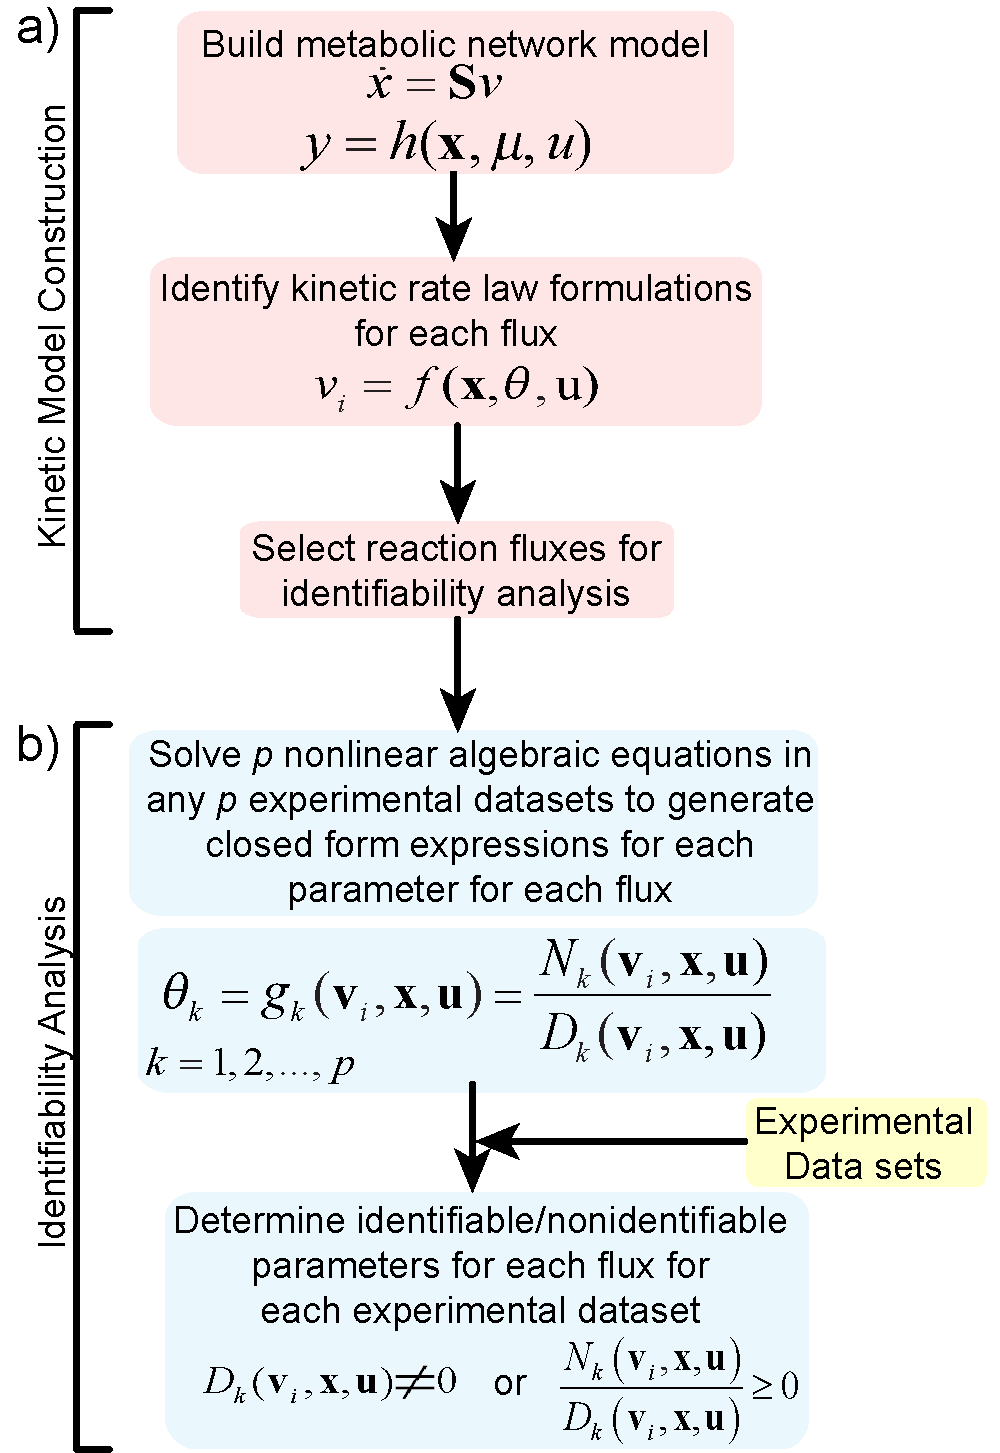
\includegraphics[width=.6\textwidth,height=.6\textheight,keepaspectratio]{C:/Users/shyam/Documents/Courses/CHE1125Project/Results/ident/figure3/ident_analysis}}
	\caption{A flow diagram showing the methodology developed to establish practical identifiability of parameters in kinetic models of metabolism. a) The steps for the construction of a kinetic model of a metabolic network are shown. The choice of rate law formulations to describe metabolic fluxes influences the identification methodology. The identifiability of parameters for each flux can be establish independently. b) in silico data generation to test the identifiability of a given parameter is an important step that is also required for experimental design using the proposed methodology. c) The steps for identifiability analysis for a parameters of a single flux are shown. d) If any of the proposed in silico experiments results in non-identifiability of any parameter, then the number and nature of experiments to be performed to establish identifiability of the corresponding parameter can be determined by following the steps shown.}\label{fig:ident-flowchart}
\end{figure}	

\subsection{Experimental design for parameter estimation in kinetic models of metabolism:}
The identifiability of each parameter based on each experiment indexed as $j = \{1, ..., n\}$ is established based on the methodology described previously in Section \ref{sec:ident} and demonstrated in Section \ref{sec:example}. Subsequently, for any flux $v_i$, if for any $p$ combinations of indices $j$, the experimental concentrations ($\mathbf{x}_j$) and fluxes ($\mathbf{v}_j$) do not satisfy the condition for identifiability for any parameter in $\theta\in\mathbb{R}^p$, i.e., $D_k(\mathbf{v}_i, \mathbf{x}, \mathbf{u}) = 0$ for any $k$, then at least one of the $p$ experiments needs to be changed to make a parameter $\theta_k$ identifiable. Consequently, the corresponding experiment cannot be used for parameter estimation and needs to be discarded from the set of all necessary experiments. Furthermore, another experiment from $j = \{1, ..., n\}$ needs to be selected such that parameter $\theta_k$ is identifiable. This process has to be repeated until all parameters in $\theta\in\mathbb{R}^p$ are identifiable for flux $v_i$. In doing so, we can arrive at a set of $p$ experiments that will always result in practically identifiable parameters for flux $v_i$. This analysis can be performed for each flux in a metabolic network independent of all the other fluxes. Hence, our method is theoretically scalable even to genome-scale models. We show the application of this design methodology for flux $v_2$ in the gluconeogenic model in Section.

Note that if none of the $n$ pre-selected experiments satisfy the identifiability condition, then we can design an $(n+1)^{th}$ experiment that can replace one of the experiments that causes practical non-identifiability using our methodology. 

In the following sections we provide a previously published kinetic model of a small gluconeogenic network, followed by a demonstration of our methodology to establish practical identifiability and experimental design for one of the fluxes in this network.

\subsection{Kinetic model of gluconeogenesis in E. coli:}\label{sec:small-model}
The proposed model for acetate consumption through gluconeogenesis and its corresponding kinetic model is used as a case study to illustrate the utility of identifiability analysis for the design of experiments for estimating parameters in kinetic models of metabolism. The kinetic model is described below.
\begin{equation}\label{eq:ode1}
\frac{d}{dt}pep=v_1-v_2-v_4
\end{equation}
\begin{equation}\label{eq:ode2}
\frac{d}{dt}fdp=v_2-v_3
\end{equation}
\begin{equation}\label{eq:ode3}
\frac{d}{dt}E=v_{e,max}\left(\frac{1}{1+\left(\frac{fdp}{K_{e}^{fdp}}\right)^{n_e}}\right) - d E
\end{equation}
The kinetic expressions for fluxes $v_1$ through $v_4$ are given below. The consumption of acetate through $v_1$ and conversion of \textit{pep} through $v_2$ are expressed in Equations (\ref{eq:flux1}) and (\ref{eq:flux2}) respectively using Michaelis-Menten kinetics. The acetate flux through $v_1$ is also governed by the quantity of available enzyme E. 
\begin{equation}\label{eq:flux1}
v_1 = k_{1}^{cat}E\frac{acetate}{acetate+K_{1}^{acetate}}
\end{equation}	
\begin{equation}\label{eq:flux2}
v_2 = V_{2}^{max}\frac{pep}{pep+K_{2}^{pep}}
\end{equation}
\begin{equation}\label{eq:flux3}
v_3 = V_{3}^{max}\frac{\tilde{fdp}\left(1+\tilde{fdp}\right)^3}{\left(1+\tilde{fdp}\right)^4+L_3\left(1+\frac{pep}{K_{3}^{pep}}\right)^{-4}}
\end{equation}
The allosterically regulated flux $v_3$ for the consumption of \textit{fdp} is expressed in Equation (\ref{eq:flux3}) using the Monod-Wyman-Changeux (MWC) model for allosterically regulated enzymes, where $\tilde{fdp}$ refers to the ratio of \textit{fdp} with respect to its allosteric binding constant $K_{3}^{fdp}$. The added flux $v_4$ for the export of \textit{pep} is expressed as a linear equation dependent on $pep$ in Equation (\ref{eq:flux4}).
\begin{equation}\label{eq:flux4}
v_4 = k_{4}^{cat}.pep
\end{equation}



\subsection{Data for establishing parameter identifiability in kinetic model of gluconeogenesis:}
Steady state metabolomics and fluxomics data can be gathered under different physiological conditions by either perturbing the expression levels for different enzymes within a metabolic network, or by changing the substrate concentrations under which the cells grow. The aforementioned model of gluconeogenesis has three different fluxes ($v_1$, $v_2$ and $v_3$) whose enzyme expression parameters ($V_1^{max}$, $V_2^{max}$ and $V_3^{max}$) can be perturbed to simulate the repression and over expression of the corresponding enzymes. Furthermore, the acetate concentration on which the cell is grown can also be perturbed to measure cellular response to changes in the substrate concentration. We use the in silico metabolomics and fluxomics data generated from these perturbation experiments to demonstrate parameter identification with our methodology. 

\section{Results:}
First, in Section \ref{sec:example} we demonstrate how our methodology can be applied for one of the fluxes in the gluconeogenic model. In Section \ref{sec:closedform} that follows, we discuss the ability to apply our methods to different nonlinear kinetic rate law formulations within the context of the gluconeogenic model. Then, in Section we discuss the different experimental design strategies that were found through our identifiability analysis to enable kinetic parameter estimation for the each flux in the model using steady state data. Finally, in Section we expand the application of our method to a relatively large (39 reactions) kinetic model of the red blood cell metabolism.

\subsection{Identifiability of parameters in a kinetic model of gluconeogenesis:}\label{sec:example}
Here, we demonstrate the use of our computer algebra-based methodology to establish practical identifiability of parameters for flux $v_2$ in the small model of gluconeogenesis described in Section \ref{sec:small-model}. Flux $v_2$ has two parameters, $V_2^{max}$ and $K_2^{pep}$ that need to be estimated from experimental data. Here, we assume that at least two different sets of experimental data for the concentrations and fluxes are available. We label the concentrations as ${pep}^1$ and ${pep}^2$, and the fluxes as ${v_2}^1$ and ${v_2}^2$ respectively, from each experiment. Accordingly, the nonlinear algebraic equations shown in Equation (\ref{eq:nonlineq}) can be formulated for flux $v_2$ as follows:
\begin{subequations}\label{eq:nonlin-flux2}
	\begin{align}
	{v_2}^1 = V_{2}^{max}\frac{pep^1}{pep^1+K_{2}^{pep}}\\
	{v_2}^2 = V_{2}^{max}\frac{pep^2}{pep^2+K_{2}^{pep}}
	\end{align}
\end{subequations}
Solving this simultaneous system of equations, we get two nonlinear algebraic equations in the parameters $V_2^{max}$ and $K_2^{pep}$ based on the form shown earlier in Equation (\ref{eq:theta-eq}).
\begin{subequations}\label{eq:v2_par}
	\begin{align}		
	V_2^{max} = \frac{v_2^1v_2^2(pep^1-pep^2)}{v_2^2pep^1-v_2^1pep^2}\\
	K_2^{pep} = \frac{pep^1(v_2^1pep^2-v_2^2pep^2)}{v_2^2pep^1-v_2^1pep^2}
	\end{align}
\end{subequations}
In Equation (\ref{eq:v2_par}), the denominator of the right hand side expression is used to test the identifiability of parameters $V_2^{max}$ (Equation \ref{eq:v2_par}a) and $K_2^{pep}$ (Equation \ref{eq:v2_par}b).

\subsection{Getting closed-form expressions for each flux in Kotte model:}\label{sec:closedform}
The complexity of the equations in our specific scenario is determined by the complexity of enzyme-metabolite interaction models used describe fluxes in metabolic networks. Although computer algebra systems (CAS) are capable of handling complex symbolic calculations, sometimes, the complexity of getting closed form expressions for all kinetic parameters of certain rate law formulations is too much for the CAS to overcome. We encountered this scenario in the case of the gluconeogenic model for flux $v_3$ where the kinetics of the allosterically activated reaction are described by the MWC model for allosteric regulation. In order to overcome this computational difficulty, we used a convenience kinetic rate law formulation to describe the allosteric interaction in $v_3$. We give this formulation in Section.

We believe this problem of computational tractability to occur in other complex kinetic rate law formulations as well. Examples?

\subsection{Experiments that can establish identifiability for each flux in Kotte model:}	
As indicated previously in Section, we performed different experiments by perturbing the parameters for fluxes $v_1$, $v_2$ and $v_3$ in the model. We also perturbed the input substrate concentration to collect data on the concentrations and fluxes within the network. We describe the results of using this data to establish the identifiability of various parameters in the kinetic model of the small metabolic network.

\subsection{Combinations of experiments that will enable identification of all model parameters:}
\subsection{Expanding methodology to RBC model:}



If any data generated from a perturbation experiment $i$ results in nonidentifiability, we eliminate experiment $i$ from the list of experiments that need to be performed for parameter estimation.



\begin{table}[!tbhp]
	\caption{Table showing the perturbed values of all fluxes used for parameter estimation.}
	\begin{center}				
		\begin{tabular}{ccc}
			Designation & Perturbed Fluxes & Perturbed Values\\
			\hline
			P1 & $v_1$ & 2\\
			P2 & $v_2$ & 0.2\\
			P3 & $v_3$ & 0.5
		\end{tabular}
	\end{center}	
	\label{tab:pval}
\end{table}

\paragraph{Outline:}
\begin{itemize}
	\item parameter estimation is a well developed field typically using minimization of least square error to estimate model parameters from available experimental data
	\item if parameters are structurally identifiable, it does not guarantee practical identifiability from noisy experimental data
	\item identifiability dependent on whether given datasets (outputs) for estimation can sufficiently distinguish between different parameter values
\end{itemize}

\paragraph{Sections:}
\begin{itemize}
	\item datasets required for parameter estimation in kinetic models of metabolism (methods?)		
	\item identifiability in kotte model - scalability, number of experiments required, requirements for time course data(? in the intro)		
	\item identifiability in large rbc model
\end{itemize}

\printbibliography
\end{document}


\subsection{Identifiability analysis: Definitions and Formulations}
Any nonlinear dynamical system can be represented by a set of states $\mathbf{x}$, observables $\mathbf{y}$ that are dependent on the states, parameters $\mathbf{\mu}$, and inputs $u$ as in Equation (\ref{eq:dynmodel}). 
\begin{subequations}\label{eq:dynmodel}
	\begin{align}
	\dot{\mathbf{x}} = g(\mathbf{x},\mathbf{\mu},u)\\
	\mathbf{y} = h(\mathbf{x},\mathbf{\mu},u)
	\end{align}
\end{subequations}
Identifiability concerns with the ability to determine a unique solution to the problem of estimating parameters $\mathbf{\mu}$ from given data on the system observables $\mathbf{y}$ for inputs $u$ \parencite{McLean2012}.	The identifiability of parameters in nonlinear models of physical processes can be classified into two categories: structural and practical identifiability. 

Given the nonlinear nature of this model, the function $f$ in Equation (\ref{eq:flux_gen}) can expressed, without loss of generality as,
\begin{align}\label{eq:nr_dr}
v = \frac{N(\mathbf{x},\theta)}{D(\mathbf{x},\theta)}
\end{align}

We use a profile likelihood-based approach \parencite{Raue2009a} to establish structural and practical identifiability of parameters in nonlinear kinetic models of metabolism. Briefly, the approach seeks to establish the existence/non-existence of bounds in confidence intervals for the estimates of parameters in nonlinear models. The profile likelihood is calculated based on Equation (\ref{eq:pl}) for each parameter $\theta_i$ where $\chi^2(\theta_i)$ is given by Equation (\ref{eq:chi2}).
\begin{align}\label{eq:pl}
\chi_{PL}^2(\theta_i) = \underset{\theta_{j\ne i}}{\mathrm{min}} \left[\chi^2(\theta)\right]
\end{align}

In the minimization objective shown in Equation (\ref{eq:chi2}) for parameter estimation, $y_{kl}^*$ is the available experimental time course data for each observable state $k$ at each $l$ time point. The difference between the data and the model estimates at these time points, $y_{kl}$ is weighted by the variance in the experimental data $\sigma_{kl}^*$. An algorithm to calculate the profile likelihood, $\chi_{PL}^2(\theta_i)$, based on Equation \ref{eq:pl} is given below.

The identifiability of parameters is established through the confidence intervals of their estimates, $\left[\sigma_{i}^-,\sigma_{i}^+\right]$. The likelihood-based confidence interval for any parameter whose profile likelihood is estimated can be written on the basis of a threshold $\Delta_{\alpha}$ in the likelihood as in Equation (\ref{eq:pleci}).
\begin{align}\label{eq:pleci}
\{\theta|\chi^2(\theta)-\chi^2(\hat{\theta})<\Delta_{\alpha}\}
\end{align}
The threshold $\Delta_{\alpha}$ in the likelihood is the 1-$\alpha$ quantile of the $\chi^2$ distribution, represented as $\chi^2(\alpha,df)$. The confidence intervals obtained hold for $df$ degrees of freedom. For a choice of $df$=1 the confidence intervals will hold for each parameter individually, and confidence intervals that hold jointly for all parameters can be obtained by choosing the number of parameters as $df$. 

The visualization of structurally and practically non-identifiable parameters using the profile likelihood approach is illustrated in Figure \ref{fig:identtypes}. The points of intersection between the profile likelihood curves (solid line) with the one parameter likelihood threshold ($\Delta_{\alpha} = \chi^2(\alpha,1)$, dashed line) provide the confidence intervals of the parameter $\theta_i$. The confidence intervals of a structurally non-identifiable parameter are unbounded, i.e., $\left[-\infty, +\infty\right]$ (Figure \ref{fig:identtypes}a), while the confidence intervals of a practically non-identifiable parameter are unbounded in at least one direction, i.e., $\left[\sigma_{i}^-,\sigma_{i}^+\right]$ where either $\sigma_{i}^- = -\infty$ or $\sigma_{i}^+ = +\infty$ (Figure \ref{fig:identtypes}b). If a parameter's estimates have a finite confidence interval then the parameter is said to be identifiable (Figure \ref{fig:identtypes}c). Note that the horizontal dotted lines in Figure \ref{fig:identtypes} represent the confidence interval thresholds ($\Delta_{\alpha}$) that are used to establish identifiability.

\begin{figure}[!tbhp]
	\centering{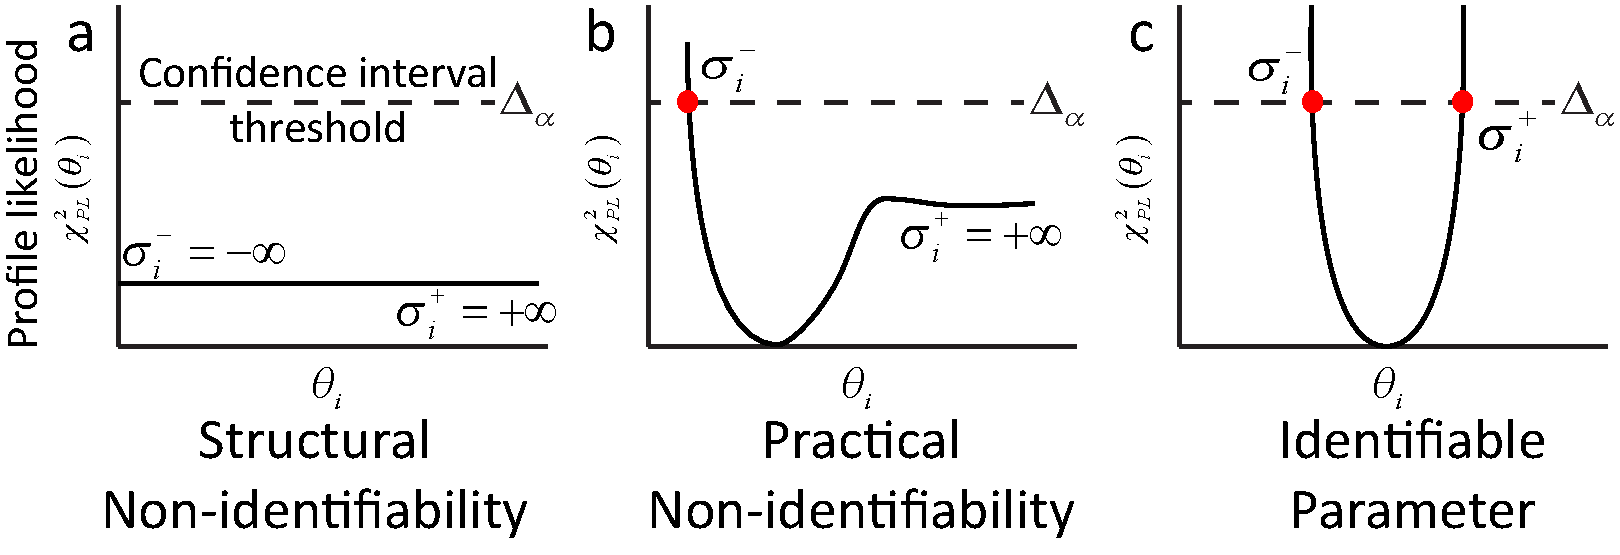
\includegraphics[width=.8\textwidth,height=.8\textheight,keepaspectratio]{figures/identifiability}}
	\caption{The profile likelihood estimates of a) a structurally non-identifiable, b) a practically non-identifiable and c) an identifiable parameter. The horizontal axis represents the changes in the value of the parameter ($\theta_i$) whose identifiability is being determined and the profile likelihood ($\chi^2_{PL}(\theta_i)$) is shown in the vertical axis. The confidence interval threshold ($\Delta_{\alpha}$) used to determine the identifiability of the parameter is denoted by the horizontal dotted line. Identifiable parameters are distinguished from non-identifiable parameters by the presence of both upper and lower bounds on their confidence interval estimates $\left[\sigma_{i}^-,\sigma_{i}^+\right]$. }\label{fig:identtypes}
\end{figure}	

Due to the dependence of practical parameter identifiability on the experimental data, the profile likelihood approach can be used to design experiments in such a way that the observables that are derived from these experiments can improve the practical identifiability of the parameters. We show how experimental design can have a meaningful impact on parameter identification and estimation in Figure \ref{fig:edwithpl}.	Assuming a parameter $\theta_i$ is practically non-identifiable (Figure \ref{fig:edwithpl}a), performing a profile-likelihood based identifiability analysis using simulated data can help determine the nature of experiments needed to make the parameter identifiable (Figure \ref{fig:edwithpl}b). In contrast, performing non-informative experiments without prior knowledge on their ability to change the identifiability of the parameter may provide data that cannot be used to estimate parameter $\theta_i$ (Figure \ref{fig:edwithpl}c).	

%Thus, the identifiability of parameters in nonlinear models is dependent on the model structure, parameterization, and the quality and quantity of experimental data that is available for the purpose of estimation. 